%%
%% Copyright (c) 2018 Weitian LI <liweitianux@sjtu.edu.cn>
%% Creative Commons BY 4.0
%%

\chapter{射电干涉技术基础}
\label{chap:interferometry}

%=====================================================================
\section{射电天文学简介}
\label{sec:radio-astronomy}

TODO

%---------------------------------------------------------------------
\subsection{射电天文学是什么?}

TODO

%---------------------------------------------------------------------
\subsection{射电窗口}

TODO

%---------------------------------------------------------------------
\subsection{机遇和挑战}

TODO


%=====================================================================
\section{辐射理论}
\label{sec:radiation}

TODO ...
spectral brightness $I_{\nu}$

%---------------------------------------------------------------------
\subsection{亮度和流量密度}

In the radio frequency regime, the Rayleigh-Jeans approximation
always holds, therefore the spectral brightness $I_{\nu}$ can be
equivalently expressed by \emph{brightness temperature} $T_b(\nu)$
through the relation \cite{condon2016}:
\begin{equation}
  \label{eq:Tb}
  T_b(\nu) \equiv \frac{I_{\nu} c^2}{2 k_B \nu^2}.
\end{equation}

%---------------------------------------------------------------------
\subsection{黑体辐射和亮温度}

TODO


%=====================================================================
\section{天线原理}
\label{sec:antenna}

TODO

%---------------------------------------------------------------------
\subsection{辐射方向图}

TODO

%---------------------------------------------------------------------
\subsection{增益和阻抗}

TODO

%---------------------------------------------------------------------
\subsection{主瓣和旁瓣}

TODO

ERA: eq:(3.96,3.118)

%---------------------------------------------------------------------
\subsection{有效面积}

TODO

%---------------------------------------------------------------------
\subsection{互易定理}

(???) TODO

%---------------------------------------------------------------------
\subsection{天线温度}

TODO


%=====================================================================
\section{干涉仪和综合孔径}
\label{sec:interferometer}

TODO

%---------------------------------------------------------------------
\subsection{基本原理}

TODO

二元干涉仪

%---------------------------------------------------------------------
\subsection{综合孔径}

TODO

坐标系统, 优点和缺点

%---------------------------------------------------------------------
\subsection{可视度}

TODO

%---------------------------------------------------------------------
\subsection{\texorpdfstring{$uv$}{uv} 覆盖}

TODO

integration time, earth rotation, phase tracking

%---------------------------------------------------------------------
\subsection{三个波束}

antenna beam, (??? primary beam), station beam, sythesized beam (PSF)

%---------------------------------------------------------------------
\subsection{三个中心}

phase center, pointing center, delay center

phase tracking, drift scan

%---------------------------------------------------------------------
\subsection{灵敏度}

point-source sensitivity, brightness sensitivity

ERA: 3.6.3.2:confusion

%---------------------------------------------------------------------
\subsection{数字波束合成}

multi-beam, phased array, 优点和缺点

%---------------------------------------------------------------------
\subsection{脏图}

weighting (natural, uniform, robust/Briggs)

%---------------------------------------------------------------------
\subsection{CLEAN 算法}

TODO

%---------------------------------------------------------------------
\subsection{大视场成像}

$w$-term, $w$-projection, $w$-stacking


%=====================================================================
\section{主要低频干涉阵列}
\label{sec:instruments}

大型低频干涉阵列是目前测量 EoR 信号的主要设备。
近十几年以及,国内外已建成一批各具特色的低频干涉阵列,
还有若干新型干涉阵列正在兴建或准备建设。
以下对其中主要的干涉阵列作简要介绍。

%---------------------------------------------------------------------
\subsection{21CMA}

\acf{21cma} 是我国开展“宇宙第一缕曙光”探测的低频射电干涉阵列,
位于中国西部天山深处的乌拉斯台,环绕在四周的高山能提供宁静的射电环境。
\acs{21cma} 的 81 个站点呈 T 形分布在东西约 \SI{6}{\km}、
南北约 \SI{4}{\km} 的两条直线上
(\autoref{fig:21cma} 展示了沿东西方向的部分站点)。
每个站点包含 127 根对数周期天线,工作频率为 \SIrange{50}{200}{\MHz},
频率分辨率为 \SI{24.4}{\kHz},
角分辨率达 \SI{1}{\arcminute}(在 \SI{200}{\MHz} 处),
采用模拟波束合成固定观测以北天极为中心、半径约 \SI{5}{\degree} 的天区
\cite{wang2013,zheng2016}。
\acs{21cma} 已于 2006 年建设完成,并于 2009 年升级了新型低噪声放大器和
基于 \acs{gpu} 的数据采集系统,目前已积累多年的观测数据。
\acs{21cma} 作为中国主要的 \acs{ska} 探路者项目,
项目成员开发了完整的数据处理流程及软件、
提出了射频干涉探测及抑制新方法 \cite{huang2016}、
探测并编录了北天极视场内的 624 个射电源 \cite{zheng2016}。
目前,\acs{21cma} 正在改造升级数字多波束合成系统,
以实现多目标跟踪观测,掌握低频脉冲星的搜寻技术。

\begin{figure}[!htb]
  \centering
  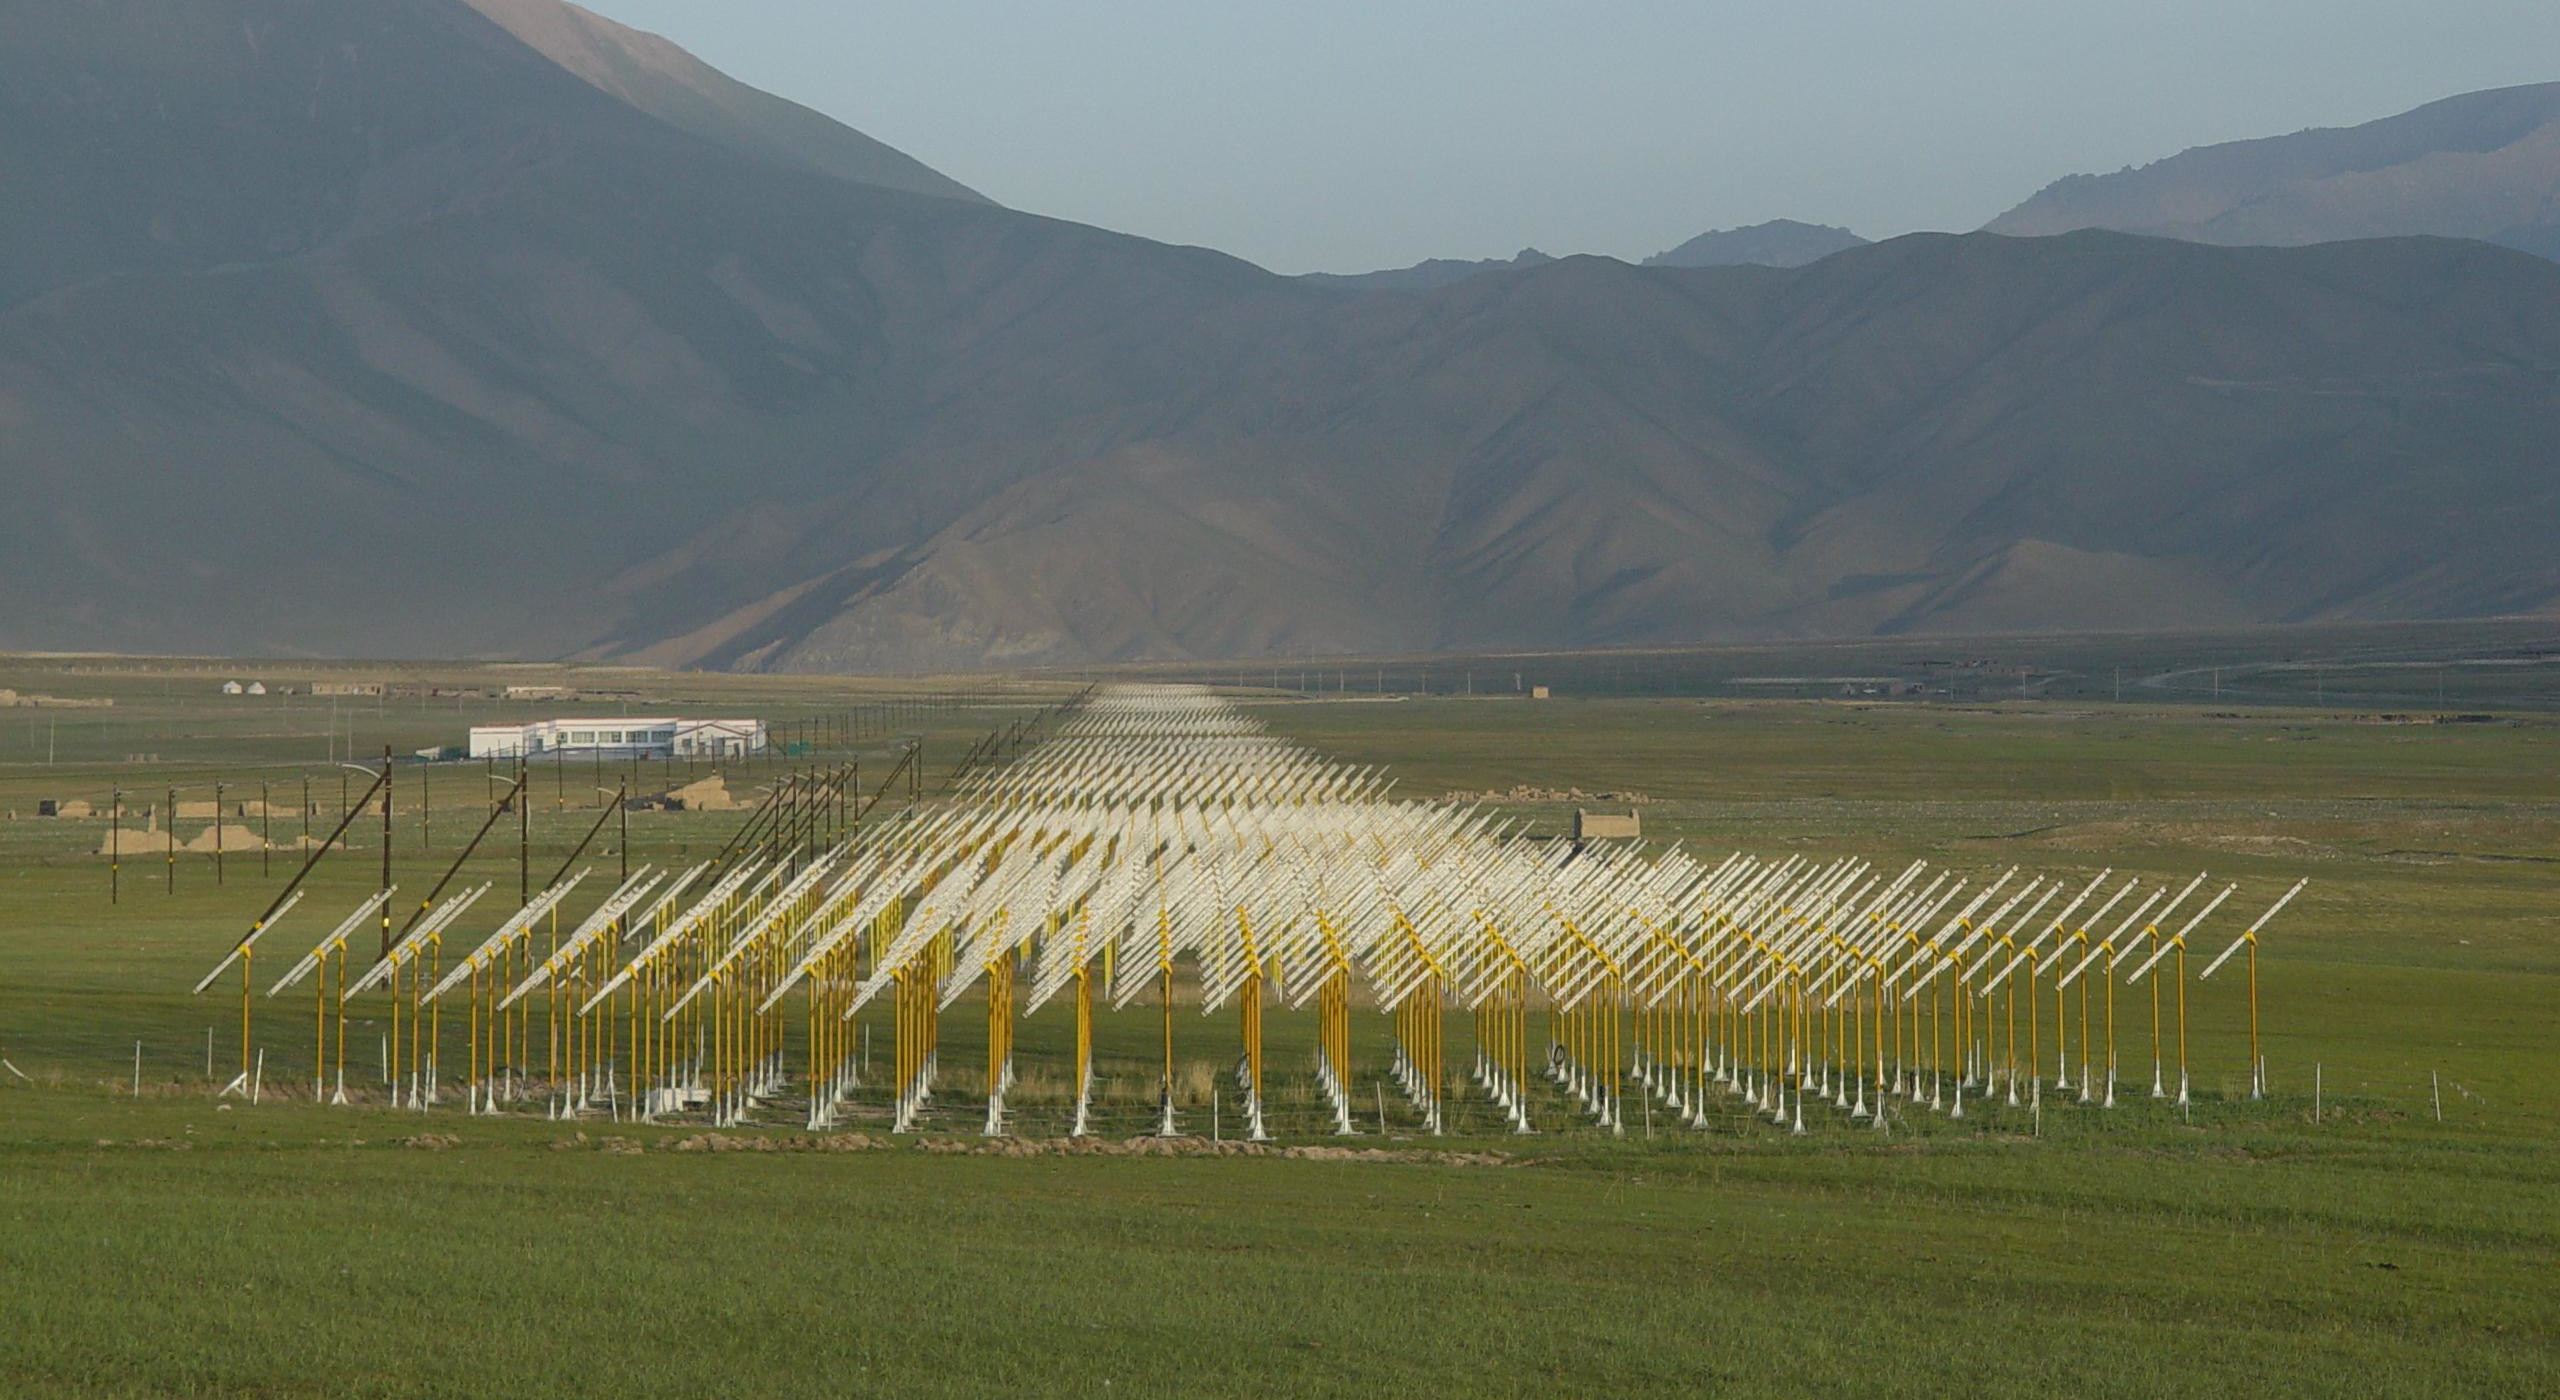
\includegraphics[width=0.8\textwidth]{21CMA}
  \bicaption[\acs{21cma} 东西方向的部分站点]{%
    \acs{21cma} 东西方向的部分站点,每个站点包含 127 根对数周期天线。
  }{%
    Part of the \acs{21cma} stations along the east-west direction,
    with each station including 127 log-periodic antennas.
    \\\textcopyright{}
    \acs{21cma}, \acl{nao}.
  }
  \label{fig:21cma}
\end{figure}

%---------------------------------------------------------------------
\subsection{LOFAR}

digital beamforming, multiple beams; SKA precursor ...

\acf{lofar} 是由\ac{astron}设计和建造的创新性的低频干涉阵列
\cite{vanHaarlem2013} (ref???),
由工作在 \SIrange{10}{90}{\MHz} 波段的低频段天线(LBA)和
工作在 \SIrange{110}{250}{\MHz} 波段的高频段天线(HBA)两部分组成。
\acs{lofar} 共有 51 个站点,
其中 24 个站点分布在半径 \SI{2}{\km} 的核心区域
(\autoref{fig:lofar} 显示了最中心的部分),
14 个站点呈螺旋状分布在外围区域,
还有 13 个国际站点分布在德国、法国、瑞士、英国、波兰和爱尔兰,
基线长达 \SI{1500}{\km}。
荷兰境内的 38 个站点各包含 96 个 LBA 和 48 个 HBA,
13 个国际站点每个包含 96 个 LBA 和 96 个 HBA。
\acs{lofar} 采用了数字多波束合成技术,能实现多目标跟踪观测,
并且显著提高巡天效率,为 \acs{ska1low} 提供强有力的技术支持
\cite{vanHaarlem2013} (ref???)。
\acs{lofar} 于 2012 年建设完成并开始观测,
已经完成北天 \SIrange{120}{168}{\MHz} 的深度巡天
\ac{lotss} \cite{shimwell2017}。
目前,\acs{lofar} 正在提议 2.0 升级计划 (ref???)。

\begin{figure}[!htb]
  \centering
  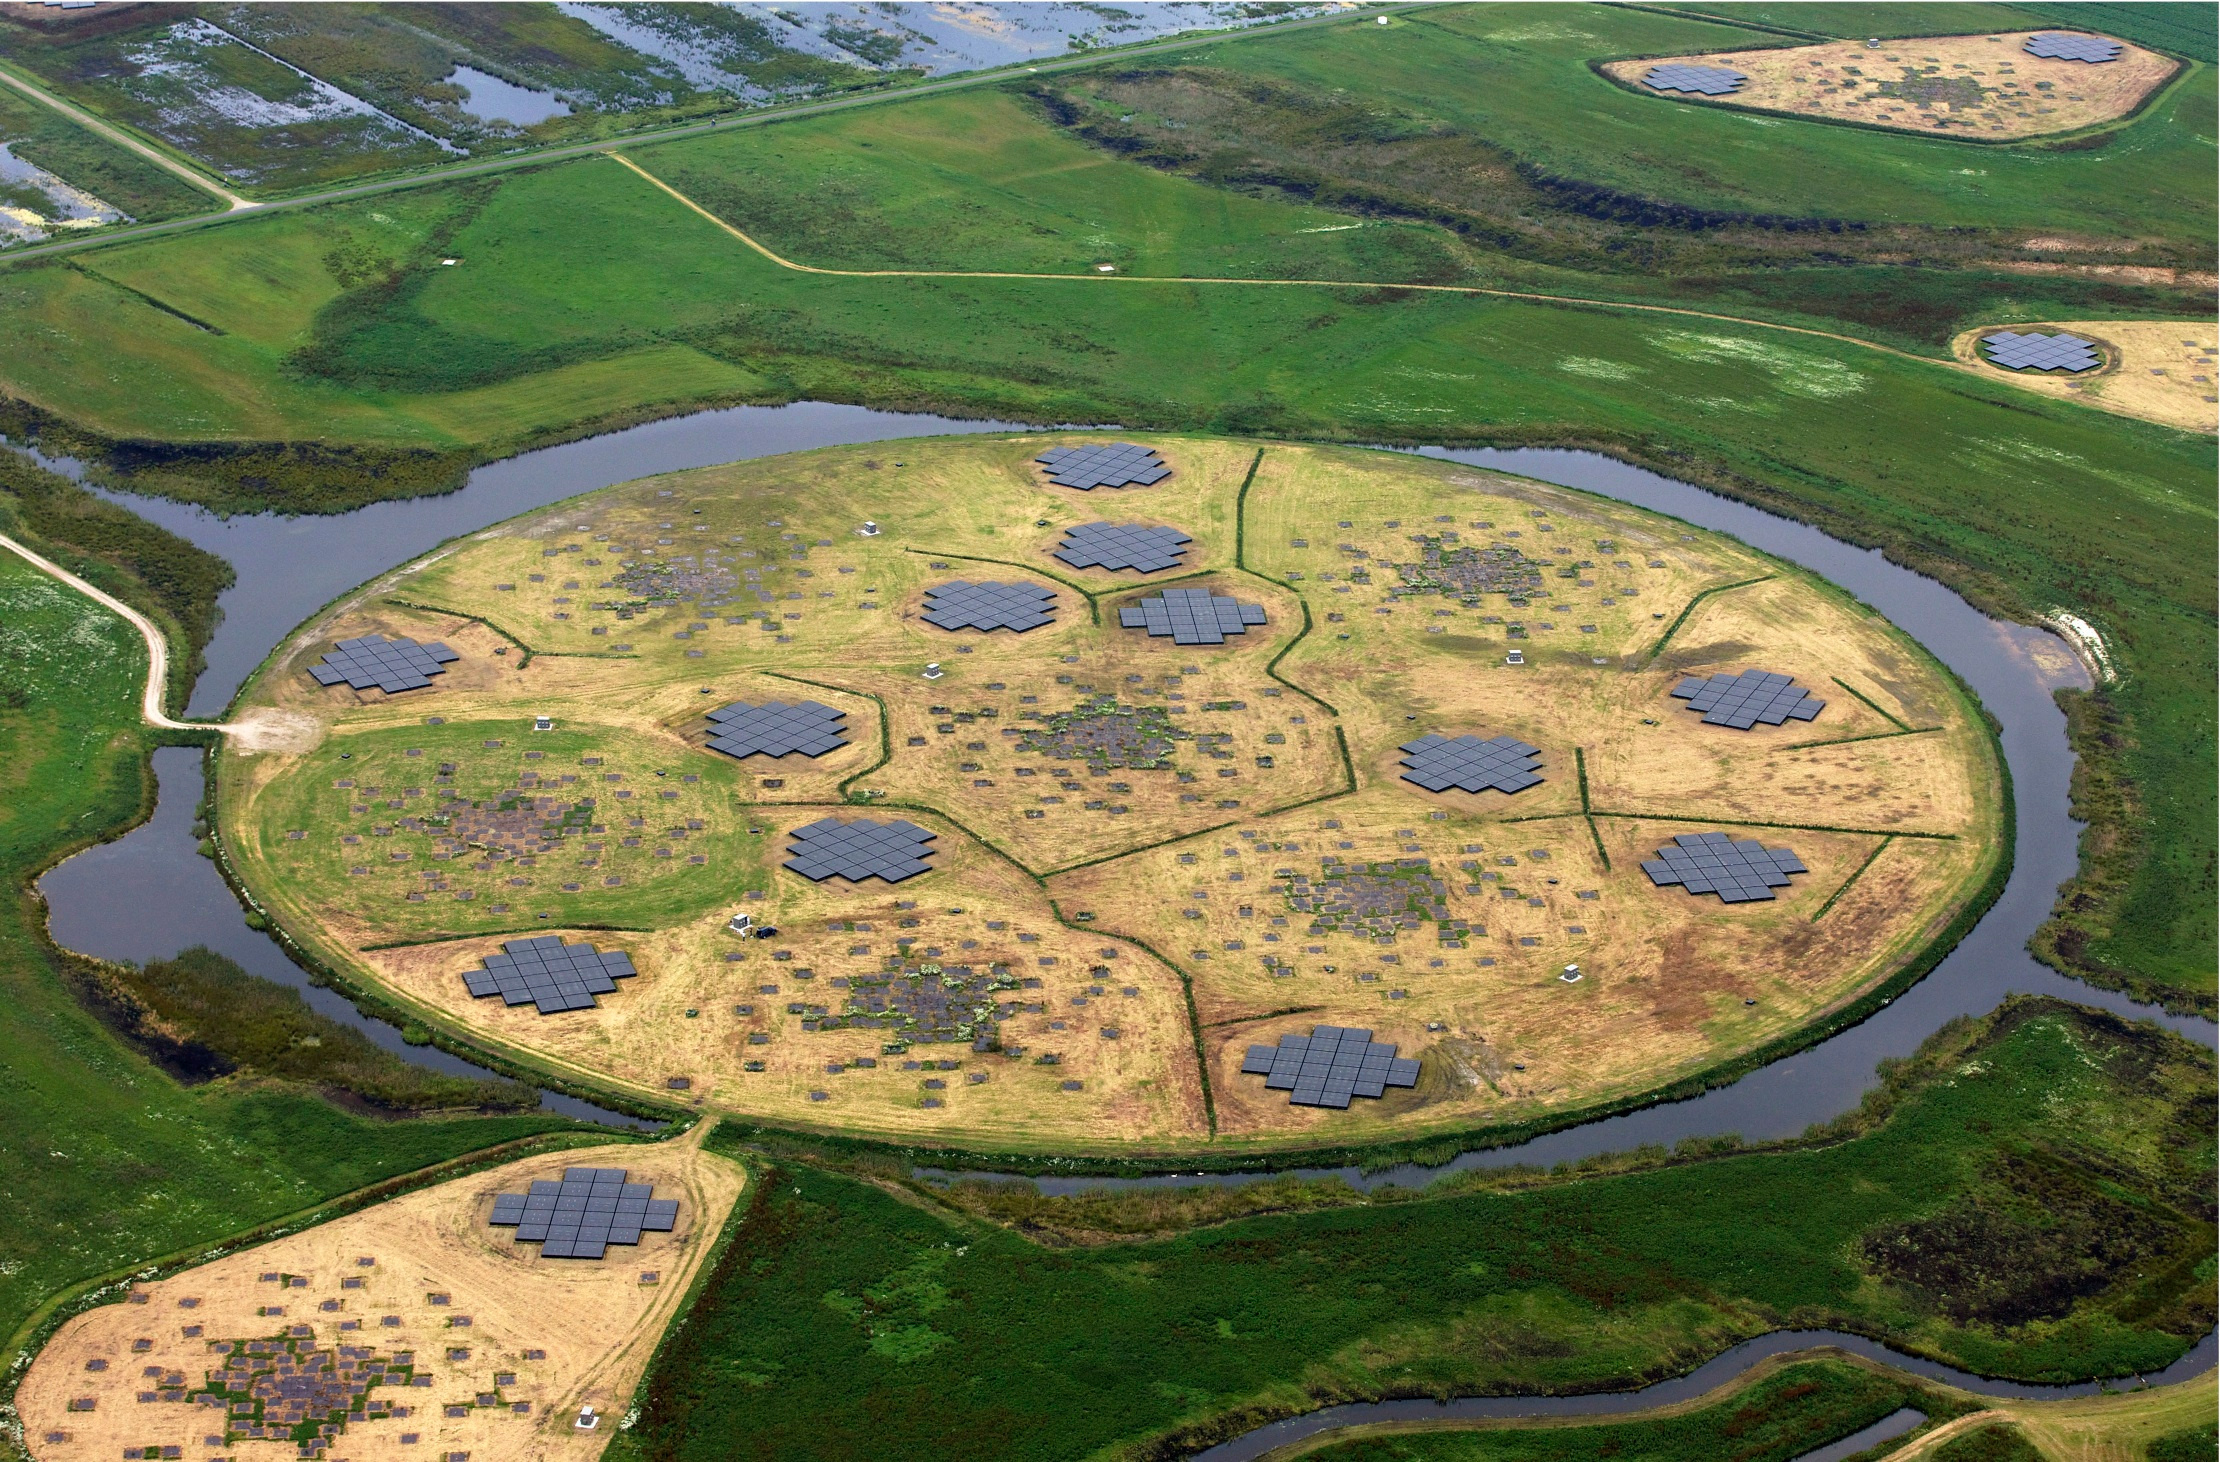
\includegraphics[width=0.8\textwidth]{LOFAR-superterp}
  \bicaption[\acs{lofar} 核心区域的中心]{%
    \acs{lofar} 核心区域的中心。
    小块深色区域为 LBA,大块深色区域为 HBA。
  }{%
    The heart of the \acs{lofar} core.
    The small dark regions are installed with LBA,
    while the big dark regions are installed with HBA.
    \\\textcopyright{}
    \textcite{vanHaarlem2013}.
  }
  \label{fig:lofar}
\end{figure}

%---------------------------------------------------------------------
\subsection{MWA}

compact + extended configurations; SKA precursor ...

\acf{mwa} 位于澳大利亚西部的 Murchison 射电天文台,
是 \acs{ska1low} 的探路者阵列 \cite{bowman2013,tingay2013}。
该阵列的主要科学目标包括宇宙再电离信号探测、河内及河外射电源、暂现源和空间天气研究。
\acs{mwa} 工作在 \SIrange{80}{300}{\MHz} 频段,使用一种双极化偶极子天线,
每个站点包含 16 个天线(按 4 行 4 列规则排列)。
所有天线均固定指向天顶,工作时通过调控各天线的时延来控制波束合成与指向。
\acs{mwa} 的特点为大视场和高表面亮度灵敏度 (???)。
\acs{mwa} 自 2007 年开始建设,于 2012 年完成了一期 128 个站点的建设,
于 2017 年底完成了二期 128 个新站点的扩建工作,目前已投入使用。
\autoref{fig:mwa} 显示了 \acs{mwa} 东侧六边形区域内的站点。
使用 \acs{mwa} 一期完成的 \ac{gleam} 巡天项目已发布一批成果,
包括点源目录 \cite{hurleyWalker2017}。。。
使用 \acs{mwa} 二期开展的 \ac{gleam-x} 巡天也正在积极进行 (ref???)。
作为少有的覆盖南天的低频射电巡天,\acs{gleam} 和 \acs{gleam-x}
将为 \acs{ska1low} 的巡天工作提供校准指导和星表的交叉认证。
同时 \acs{mwa} 也将会为 \acs{ska1low} 的宇宙再电离探测任务提供
更精准的天空模型和天区指导。

\begin{figure}[!ht]
  \centering
  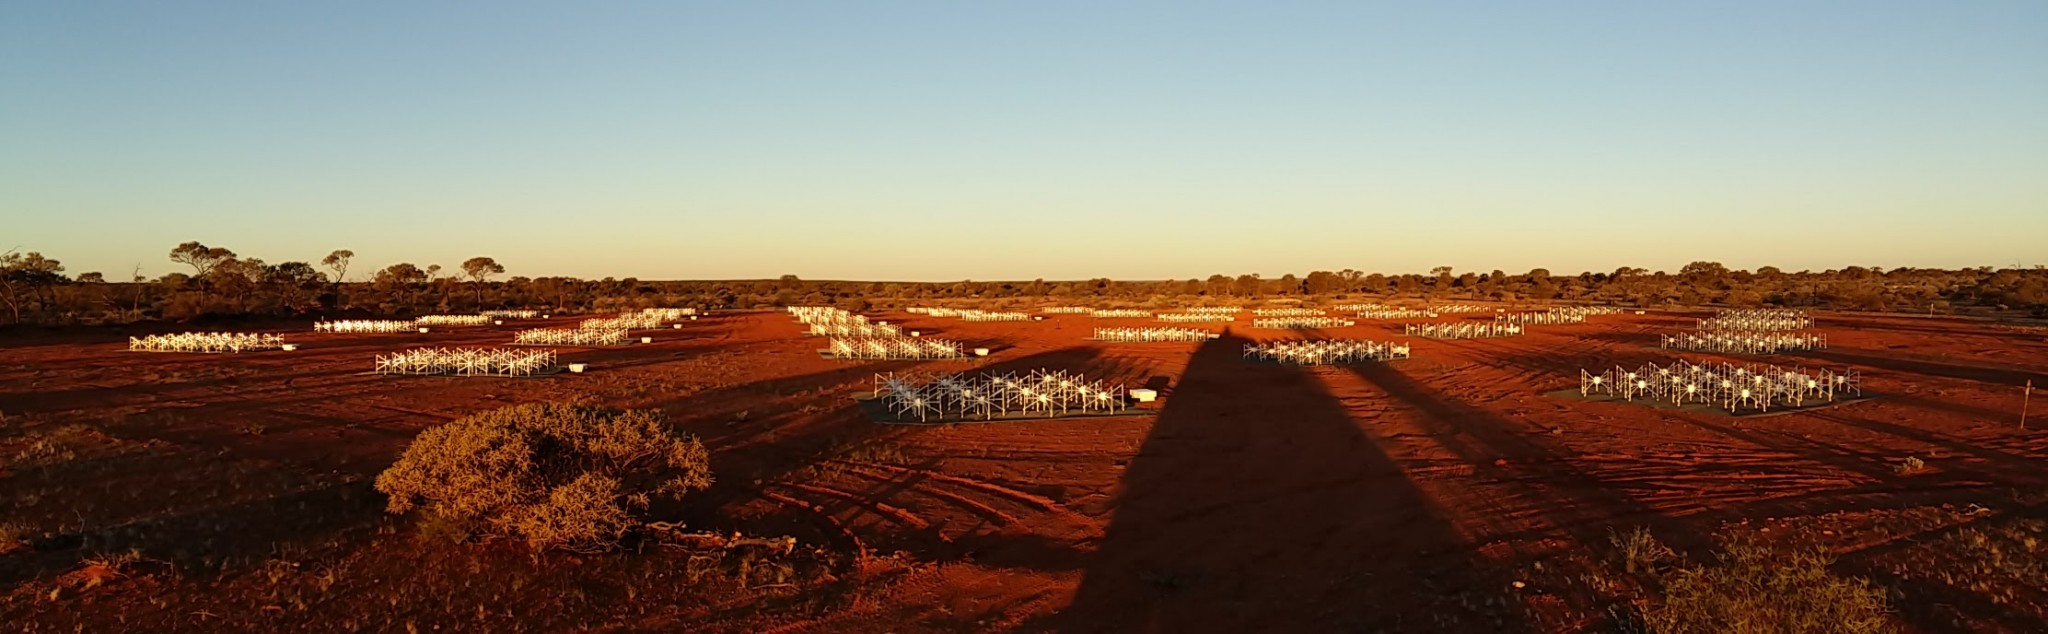
\includegraphics[width=\textwidth]{MWA}
  \bicaption[\acs{mwa} 东部站点]{%
    \acs{mwa} 东侧六边形区域内的站点,每个站点包含 16 个天线。
  }{%
    The stations inside the \acs{mwa}'s east hexagonal region,
    with each station consisting of 16 antennas.
    \\\textcopyright{}
    \acuse{icrar}\ac{icrar}/\acs{mwa},
    \url{https://www.icrar.org/multimedia/images/}, (2018-10-04).
  }
  \label{fig:mwa}
\end{figure}

%---------------------------------------------------------------------
\subsection{LWA}

\acf{lwa} 是一个正在建设于美国新墨西哥州中部的大型低频干涉阵列,
计划由 53 个分布远达 \SI{400}{\km} 的站点组成,
每个站点的大小约 \SI{100x100}{\meter} 并且包含 256 个双极化天线,
总接收面积达 \SI{1}{\km\squared}(在 \SI{10}{\MHz} 处),
工作在非常低频的 \SIrange{10}{88}{\MHz} 波段,
这是我们目前了解最少的射电波段 \cite{ellingson2009}。
借助其高灵敏度和高角分辨率,\acs{lwa} 将打开这一个新射电窗口,
研究宇宙高能粒子加速机制、早期宇宙及其演化、暂现源、银河系星际介质、
太阳活动及电离层性质等。
\acs{lwa} 所采用的大站点设计使其更适合研究银河系的大尺度结构。
\acs{lwa} 的首个站点(LWA1;\autoref{fig:lwa})位于 \ac{vla} 附近,
已于 2009 年建设完成,并于 2011 年开始正式观测 \cite{taylor2012,ellingson2013};
其他站点正在积极建设之中。
\acs{lwa} 亦采用数字波束合成技术,但其创新之处在于每个站点均可独立使用并成像。
目前已使用 \acs{lwa}1 开展巡天并获得了 \SIrange{35}{80}{\MHz}
北天图像 \cite{dowell2017}。

\begin{figure}[!htb]
  \centering
  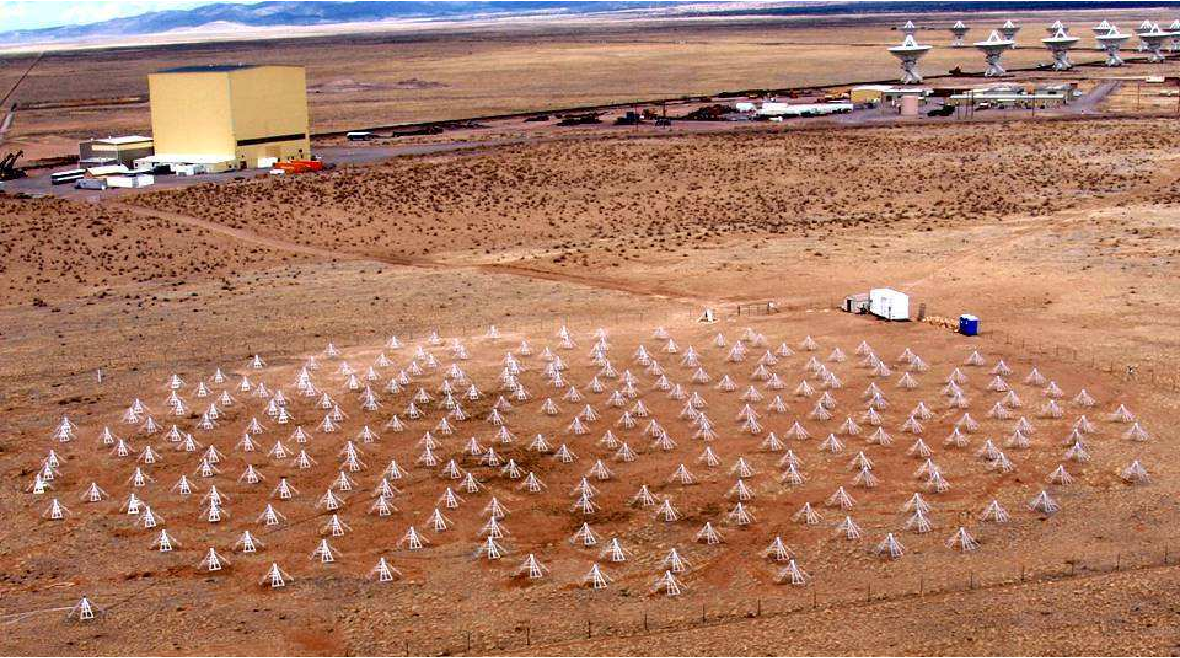
\includegraphics[width=0.8\textwidth]{LWA1}
  \bicaption[\acs{lwa} 的首个站点(LWA1)]{%
    位于 \acs{vla} 附近的 \acs{lwa} 的首个站点(LWA1),包含 256 个天线。
  }{%
    The first station of \acs{lwa}, i.e., LWA1,
    which locates near the \acs{vla} and contains 256 antennas.
    \\\textcopyright{}
    \textcite{taylor2012}.
  }
  \label{fig:lwa}
\end{figure}

%---------------------------------------------------------------------
\subsection{MITEoR}

\acf{miteor} 是一个使用\ac{fftt} 新技术\cite{tegmark2009}的先导阵列,
由 64 个按 8 行 8 列规则分布的全同双极化天线构成(\autoref{fig:miteor}),
在 \SIrange{100}{200}{\MHz} 范围内覆盖两个宽度为 \SI{25}{\MHz} 的频段
\cite{zheng2014}。
利用这种天线布局方式,可以直接对天线采集信号运用\ac{fft}进行成像,
避免了传统干涉阵列耗时的天线间两两相关运算,
将计算复杂度由 $O(N_{\!A}^2)$ 显著降为 $O(\acs{N-ant} \log\acs{N-ant})$,
其中 \acs{N-ant} 为\acl{N-ant},
同时还将数据存储压力从 $O(N_{\!A}^2)$ 大幅减轻至 $O(\acs{N-ant})$。
如此可以极大地降低建设和运行成本,非常有利于建设超大规模的干涉阵列,
实现极高的灵敏度,使观测者在更大的红移范围上更准确、更多地探知
宇宙中物质分布的功率谱模式。
此外,阵列中的大量冗余基线能为系统自校准提供有效帮助 \cite{dillon2016}。
目前,\acs{miteor} 已开展观测并公布了 \SIrange{128}{175}{\MHz} 的北天图像
\cite{zheng2017},充分验证了 \acs{fftt} 技术的可行性,
该技术的创新性和巨大潜力能在未来 EoR 实验中发挥重要作用。

\begin{figure}[!htb]
  \centering
  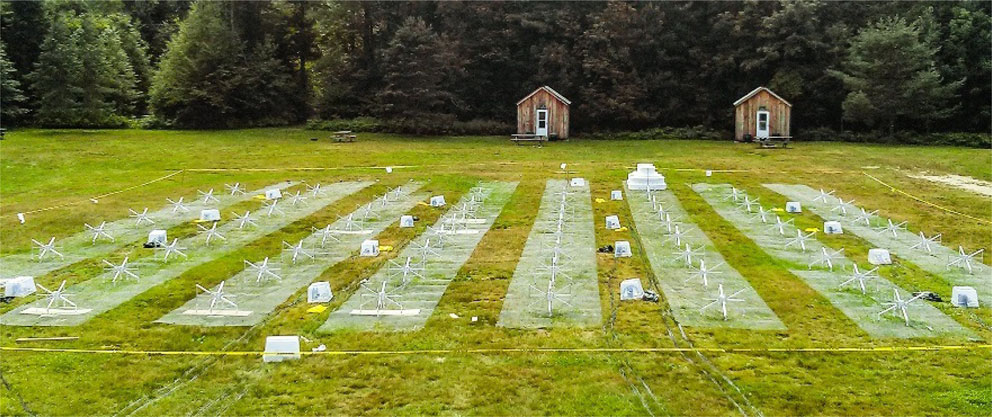
\includegraphics[width=\textwidth]{MITEoR}
  \bicaption[\acs{miteor} 干涉阵列]{%
    在 2013 年夏天部署完成的 \acs{miteor} 干涉阵列,
    64 个双极化天线规则地分布在 \SI{21x21}{\meter} 的矩形区域,
    相互之间分隔 \SI{3}{\meter}。
  }{%
    The \acs{miteor} array deployed in the summer of 2013.
    The 64 dual-polarization antennas were laid on a \SI{21x21}{\meter}
    regular grid with a separation of \SI{3}{\meter}.
    \\\textcopyright{}
    \textcite{zheng2014}.
  }
  \label{fig:miteor}
\end{figure}

%---------------------------------------------------------------------
\subsection{HERA}

\acf{hera} 由美国在南非 Karoo 射电天文保护区建造,
可被视为继 \acs{mwa}、\ac{paper} 等低频射电探路者阵列之后
设计和技术趋于成熟的第二代宇宙再电离时期探测阵列 \cite{deboer2017}。
该阵列由一个尺寸为 \SI{300}{\meter} 的正六边形核心区以及外围区构成。
核心区中规则地布置了 320 面直径为 \SI{14}{\meter} 的固定式抛物面碟形天线,
外围区则分散布置 30 面同样的天线。
\autoref{fig:hera} 显示了 \acs{hera} 已于 2016 年建成的 19 面天线。
\acs{hera} 的观测频率为 \SIrange{50}{250}{\MHz},
首要科学目标是通过研究天空信号二维功率谱的 EoR 窗口(详见 \autoref{sec:eor-window})
精确测量再电离信号,描绘宇宙再电离时期以及之前的宇宙大尺度结构。
\acs{hera} 的阵型和天线设计保证了它能够为 EoR 信号的观测提供高灵敏度、
易于借助大量冗余基线进行系统校准 \cite{dillon2016}、
在需要时可启用 \acs{fftt} 观测模式(虽然阵列中的天线数目并不庞大)\cite{tegmark2009}。
由此带来的主要弱点是角分辨率较低、能够测量的功率谱模式较少、栅瓣效应较明显 (ref???)。
目前 \acs{hera} 的第一期 37 面天线已经安装完毕并开始试观测,
第二期的 128 面天线也已开始建设,是 \acs{ska1low} 的有力竞争者。

\begin{figure}[!htb]
  \centering
  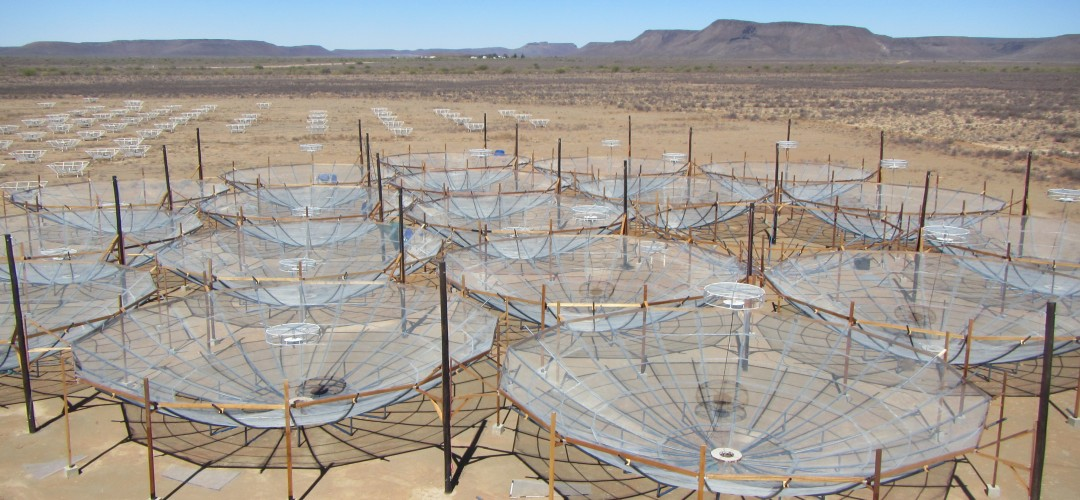
\includegraphics[width=\textwidth]{HERA19}
  \bicaption[\acs{hera} 已建成的 19 面天线]{%
    \acs{hera} 在 2016 年建成的 19 面碟形天线。
    后方的小型天线属于 \acs{paper} 项目。
  }{%
    The \acs{hera}'s 19 dish antennas deployed in South Africa in 2016.
    The small antennas in the background belong to the \acs{paper}
    experiment.
    \\\textcopyright{}
    \acs{hera}/SKA Africa, \url{http://reionization.org/}, (2018-10-04).
  }
  \label{fig:hera}
\end{figure}

%---------------------------------------------------------------------
\subsection{SKA}

TODO


%=====================================================================
\section{小结}

TODO


%% EOF
